\chapter{Результаты работы программы}

Для Варианта №10

\begin{itemize}[label=]
    \item \textbf{Точечные оценки:}
    \begin{itemize}[label=]
        \item $\hat\mu (\vec x_n)$ = 1.836
        \item $S^2(\vec x)$ = 1.153
    \end{itemize}
    \item \textbf{$\gamma$-доверительные интервалы при} $\gamma$=0.9:
    \begin{itemize}[label=]
        \item $(\underline\mu (\vec x_n), \overline\mu (\vec x_n))$ = (1.6739, 1.9989)
        \item $(\underline\sigma^2 (\vec x_n), \overline\sigma^2 (\vec x_n))$ = (0.9430, 1.4467)
    \end{itemize}
\end{itemize}

\begin{figure}[h]
	\centering
	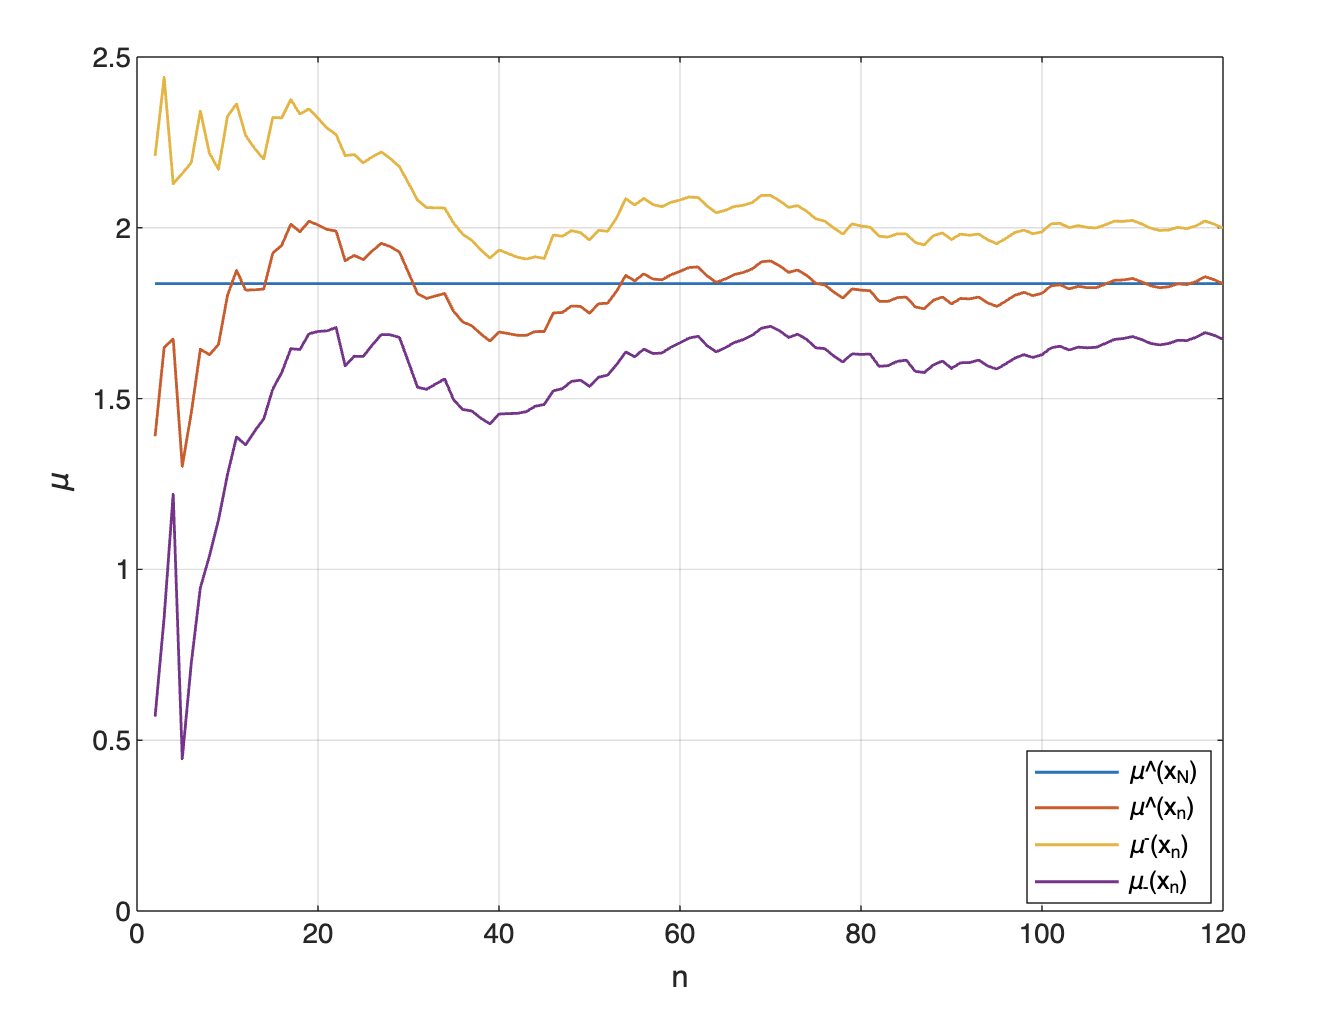
\includegraphics[scale=0.75]{images/mu.png}
	\caption{График зависимости оценки математического ожидания и границ $\gamma$-доверительного интервала от объема выборки $n$}
	\label{fig:histo}
\end{figure}

\begin{figure}[h]
	\centering
	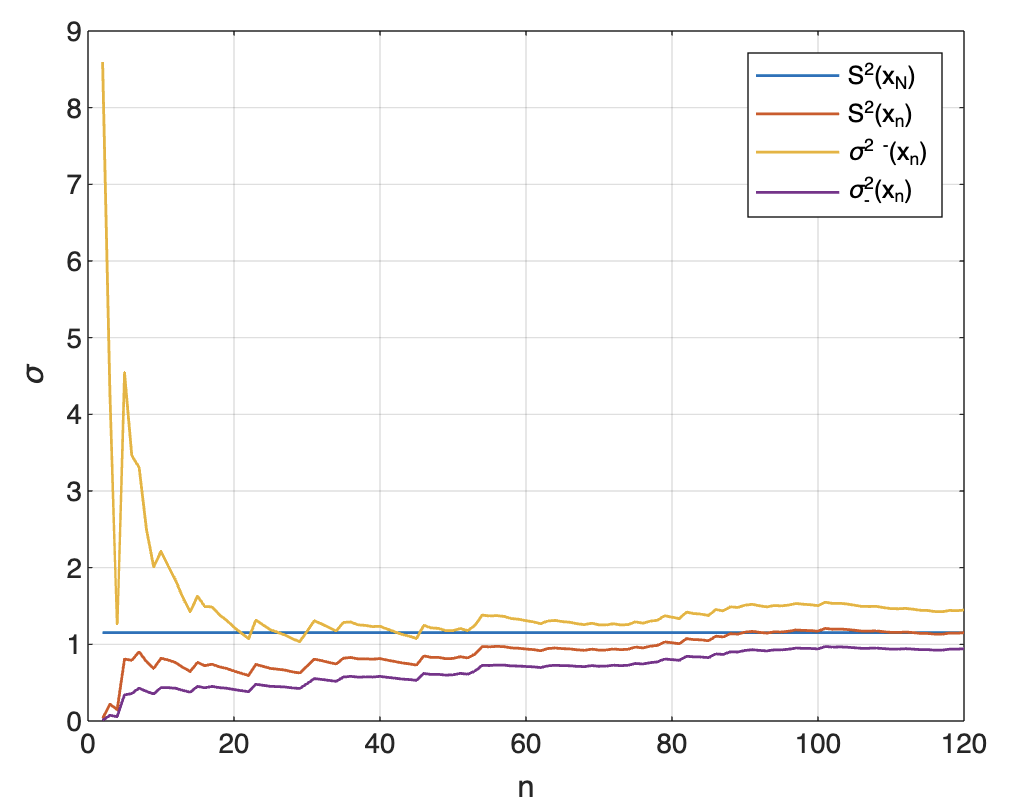
\includegraphics[scale=0.9]{images/sigma_square.png}
	\caption{График зависимости оценки дисперсии и границ $\gamma$-доверительного интервала от объема выборки $n$}
	\label{fig:emperic}
\end{figure}
